\documentclass[a4paper, oneside, 10pt]{book}

\usepackage{fancyhdr,verbatim, listings, color} 
\usepackage{shorttoc}
\usepackage[french]{minitoc}
\usepackage[pdftex]{graphicx} 
\usepackage[utf8]{inputenc}
\usepackage[T1]{fontenc}
\usepackage[frenchb]{babel}
\usepackage{amsmath,amssymb,mathrsfs}
\usepackage[french]{varioref}
\usepackage{url}
\usepackage{../nota}
\usepackage{../citation}
%\usepackage{../sommaire}

\graphicspath{%
  {../imgs/}%
  {imgs/}
}

% NOTES
\setlength{\largeurnota}{.8cm}
\newenvironment{attention}{%
  \begin{pictonote}{attention}}{\end{pictonote}}
\newenvironment{note}{%
  \begin{pictonote}{note}}{\end{pictonote}}
\newenvironment{question}{%
  \begin{pictonote}{question}}{\end{pictonote}}

\usepackage[pdftex=true,
    bookmarks         = true,
    bookmarksnumbered = true,
    bookmarks = true, 
    pdfstartview      = FitH,
    bookmarksopen     = true, 
    bookmarksopenlevel = 1, 
    hyperindex        = true,
    colorlinks        = true,
    %urlcolor          = red,
    %pdfborder         = {0 0 0}
    ]{hyperref}

\definecolor{colKeys}{rgb}{0,0,1} 
\definecolor{colIdentifier}{rgb}{0,0,0} 
\definecolor{colComments}{rgb}{0,0.5,1} 
\definecolor{colString}{rgb}{0.6,0.1,0.1} 

\lstset{
float=hbp,
basicstyle=\ttfamily\small,
identifierstyle=\color{colIdentifier},
keywordstyle=\color{colKeys},
stringstyle=\color{colString},
commentstyle=\color{colComments},
language=c++,
columns=flexible,
tabsize=2,
frame=trBL,
frameround=tttt,
extendedchars=true,
showspaces=false,
showstringspaces=false,
numbers=left,
numberstyle=\tiny,
breaklines=true,
breakautoindent=true,
captionpos=b,
commentstyle=\textit
}

\lstnewenvironment{cpp}{\lstset{language=c++}}{}

%% Define a new 'leo' style for the package that will use a smaller font.
\makeatletter
\def\url@leostyle{%
  \@ifundefined{selectfont}{\def\UrlFont{\sf}}{\def\UrlFont{\small\ttfamily}}}
\makeatother
%% Now actually use the newly defined style.
\urlstyle{leo}

\pagestyle{fancy} 



\hypersetup{
    pdfauthor   = {Arnaud Audoin, Clément Badiola, Samuel Da Silva, Alexandre Perrot, Camille Ritlewski},% 
    pdftitle    = {PER - Rapport final},%
    pdfsubject  = {Rapport final},% 
    pdfkeywords = {},% 
    pdfcreator  = {PDFLaTeX},% 
    pdfproducer = {PDFLaTeX}} 

\author{Arnaud~\textsc{Audoin} \and Clément~\textsc{Badiola} \and Samuel~\textsc{Da~Silva} \and Alexandre~\textsc{Perrot} \and Camille~\textsc{Ritlewski} \and \\
  Client : Paul~\textsc{Dorbec}}
\title{The map coloring game \\ Final report}
\date{24 janvier 2013}

\begin{document}

\graphicspath{{../imgs/}}

\fancyhf{} 
\renewcommand{\chaptermark}[1]{\markboth{#1}{}} 
\renewcommand{\sectionmark}[1]{\markright{\thesection\ #1}} 
\fancyhead[R]{\bfseries\thepage}% Left Even, Right Odd - No de page 
\fancyhead[L]{\bfseries\rightmark} % Left Odd - Titre section 
\renewcommand{\headrulewidth}{0.5pt}% filet en haut de page 
\addtolength{\headheight}{0.5pt} % espace pour le filet 
\renewcommand{\footrulewidth}{0pt} % pas de filet en bas 
\fancypagestyle{plain}{ % pages de tetes de chapitre 
  \fancyhead{} % supprime l’entete 
  \renewcommand{\headrulewidth}{0pt} % et le filet 
}

\fancypagestyle{plain}{
	\fancyhf{}
	\fancyfoot[C]{\thepage}
	\renewcommand{\headrulewidth}{0pt}
	\renewcommand{\footrulewidth}{0pt}}

\dominitoc

\maketitle

\frontmatter

%Phrase d'accroche (problématique principale et objectif principal) + résumé des moyens employés (listing) + résumé vague des conclusions obtenus.
\chapter{Problème}
\minitoc

%\input{sections/probleme_exemple}
 %Enoncé du problème et des objectifs puis résumé (synthèse d'une page max.) du projet

\tableofcontents

\mainmatter

\chapter{Introduction}

Texte ici. 

\vfill

\textbf{Mots-clés :} mot clef 1, mot clef 2, macFly

\vfill
 %Définir le probleme, les objectifs, le cadre de travail (contexte).


%l'état de l'art se trouve dans l'introduction
%\chapter{Documentation}
\minitoc

%\section{Historique}
\section{Historique}

\begin{description}
\item[1940] Invention de la loupe téléscopique.
\item[1943] McFly et Marty inventent la voiture à remonter le temps. 
\end{description}

Depuis, les recherches sur les sulfatrons pulsatifs ionisés n'ont cessé d'amener de nouvelles applications, en combinant parfois plusieurs modèles.




%\section{Modèles courants}
\input{sections/dom_modeles}

%\section{Utilisations}
\section{Utilisations}

De part leur fort potentiel pour résoudre des problèmes de nature biotroniques, les produits lactiques représentent un secteur de recherche très attractif pour les PME. Voilà.



 %etat de l'art (contexte technique et scientifique), bibliographie importante.

%%%%%% Stratégies tirées de l'article
\chapter{Theory}

To understand the strategies that follow, we first introduce three important concepts:
\begin{itemize}
\item the order of a graph $G$
\item the loose backward neighbors
\item the number of 2-coloring of a graph $G$, denoted $col_{2}(G)$
\item the chromatic number of a graph $G$, denoted $\chi(G)$
\item the game chromatic number of a graph $G$, denoted $\chi_{g}(G)$
\end{itemize}


The chromatic number of a graph $G$ is the minimum number of colors to make a good coloring of $G$.

The game chromatic number is the number of allowed colors for which Alice always has a winning strategy.

The order of a graph $G$ is a linear representation of the vertices of the graph where we associate an index to each vertex according to its position in the order.

\includegraphics[width=13cm]{IntroOrder.jpg}

For the loose backward neighbor, we define an order of the graph $G$: $v_{1} v_{2} v_{3}... v_{n}$. A vertex $v_{h}$ is a loose backward neighbor of $v_{i}$ if $h < i$ and if $v_{h}$ is in $v_{i}$ neighborhood, or if $v_{h}$ and $v_{i}$ have a common neighbor $v_{j}$ such as $ h < i < j$.

\includegraphics[width=7cm]{looseIntro.jpg}

Now, let's review the whole range of orders for a graph $G$. For each order found, we determine the integer $k$ such as each vertex of the order has a number of loose backward neighbors $<$ to $k$. We keep the order which has the smallest $k$. This $k$ is the number of 2-coloring. In addition, the associated order satisfies $col_{2}(G)$.

\section{First strategy}

Alice determines a sequence of vertices of the graph $G$ satisfying $col_{2}(G)$. The game begins only after.

\includegraphics[width=13cm]{IntroOrder.jpg}
\includegraphics[width=10cm]{Orderstep.jpg}

When Bob colors a vertex $v_{h}$,
Alice's strategy is to seek in the order previously determined the loose backward neigbor of $v_{h}$ not yet
colored having the lowest index. Once found, it is colored. If Alice does not find such a vertex, she simply picks from the uncolored vertices set the one with the lowest index in the order.
According to this strategy, each graph $G$ satisfies $\chi_{g}(G) \leq \chi(G) \times (1 + col_{2}(G))$.
\section{Second strategy}

As in the previous strategy, Alice will once again need an order satisfying $col_{2}(G)$.
Using this order, she will achieve her own coloring of the graph (without any intervention from Bob).
This coloration must comply with the following rules:
\begin{itemize}
\item A vertex must not have the same color as its loose backward neighbors.
\item Vertices forming a cycle must be colored with at least 3 colors.
\item This coloring must use at most $col_{2}(G)$ colors.
\end{itemize}

We will call the resulting graph $G'$.

\includegraphics[width=13cm]{gameS2t1.jpg}

Now Alice will use $G'$ to provide guidance in the coloring of the graph $G$. For each bicolor subgraph of $G'$,
we direct the edges such that each vertex has an out-degree of no more than $1$. 

\includegraphics[width=8cm]{gameS2t2.jpg}

As each edge appears only in
one subgraph, we know that we oriented the entire graph $G$. We can now begin the game. 
A vertex $v$ (colored with a color $c$ on the graph $G'$) is endangered if one of its incoming neighbors is colored in a shade of $c$. Alice coloring the graph in accordance with the coloring of $G'$, a vertex can only be endangered by Bob. In addition, the orientation of $G'$ is such that there can be only one vertex in danger per round.

\includegraphics[width=8cm]{gameS2t3.jpg}

According to this strategy, each graph satisfies $\chi_{g}(G) \leq a(G) \times (a(G) + 1)$, where $a(G)$, the acyclic chromatic number of $G$, is the minimum number of colors used on $G$ such that each cycle is colored with at least $3$ colors.
\section{Third strategy - Daltonism may help}

As with previous strategies, we order the vertices according to $col_{2}(G)$.
We would like to draw your attention to the fact that we no longer use the loose backward neighbors, just the backward neighbors, ie neighbors with a lower index in the order.

In this case, we use a rather simple activation strategy.
When Bob colors a vertex $v$, Alice begins by activating the vertex $v$, then she checks its backward neighbors.
$x$ is the backward neighbor of $v$ having the lowest index in the order.
If $x$ is colored, we turn to the next backward neighbor of $v$. If $x$ is activated, then it is in danger and we immediatly give it a color. If $x$ is not activated, then we activate it and we check its backward neighbors. If x has no unshaded backward neighbor, then we color $x$.
In the case in which the vertex v (colored by Bob) has no unshaded backward neighbor, then we color the unshaded vertex having the lowest index in the order previously calculated.


According to this strategy, each graph satisfies $\chi_{g}(G) \leq 3 \times col_{2}(G) - 1$.
\section{Fourth strategy}

The purpose of this strategy is to find a better ordering of the graph $G$, on which we will use the activation strategy previously seen. We construct this order inductively (i.e. in the reverse order). The first selected node will be any vertex of $G$ with a degree of at most $5$.
Suppose we have already taken the vertices $v_{n}, v_{n-1}, ..., v_{i+1}$ except $v_{i}$ and we seek a candidate for $v_{i}$:

We split the vertices of $G$ into two parts: $C = (v_{n}, v_{n-1}, ..., v_{i+1})$ and $U = V \setminus C$.
We construct a new graph $H$ as follows:
\begin{itemize}
\item We remove the edges between the vertices of C.
\item We remove each vertex $v$ of $C$ having at most three adjacent vertices in $U$.
\item For each vertex $v$ removed, we add edges between its neighbors in $U$ in order to form a clique.
\end{itemize}

Now that we have our graph $H$, we assign to each edge $e$ 2 dollars (USD) spread over its vertices as follows:
\begin{itemize}
\item If $e$ connects two vertices of $U$, we give \$ 1 to each vertex of $e$.
\item If $e$ connects $x$ in $U$ and $y$ in $C$, then we give \$ 0.50 to $x$ and \$ 1.50 to $y$.
\end{itemize}

Once we have distributed the USD, we need to find a single vertex with a total value of less than \$ 6.
It will be our $v_{i}$.

When we have our order, we use the color-blind activation strategy on it.

According to this strategy, each graph satisfies $\chi_{g}(G) \leq 18$.
 %théorie spécifique à notre probleme (les differents théoremes) (les détails seront a mettre en annexe).

\chapter{Work}
\minitoc

\section{Objectives}

After the study of the article, we agreed on implementing an AI to play the game. We wanted to know how would a computer program compete against the article's theoretical bounds. The first step was to choose the type of algorithmto use for this AI. Seeing how the move space was large (we were later comforted in this idea by our complexity study), Monte-Carlo Tree Search seemed to be the best choice for it allows good decisions without exploring the entire tree. Another important constraint was our inability to evaluate the profit of a game's position for a player before the game has ended. We could therefore not use more classical AI algorithms, where the tree search is stopped at a constant depth and the game state is evaluated before its end.

\section{Monte Carlo}

Monte-Carlo methods are a set of randomized algorithms. The general idea is to use random sampling rather than computing to help solve a problem. Such algorithms are mostly used when computing a solution to the problem is not feasible. Because of the use of random sampling, they are heuristical by nature : their results are not always guaranteed to be exact. Throughout the years, Monte-Carlo methods have been successfully used in physics, mathematics  and computer science.

In this report, we will be interested in a special case of Monte-Carlo method : Monte-Carlo tree search, aka MCTS. It applies Monte-Carlo principles to tree exploration. The main field of application is artificial intelligence, especially games with very large move space where a complete tree exploration is not possible in reasonable time, such as Chess and Go.

Dans Monte Carlo, on va chercher à jouer beaucoup de parties pour un graph donné (que nous appellerons le graph étudié) afin de pouvoir jouer les meilleurs coups possibles. 
Pour chaque graph étudié, nous générons un arbre des coups joués où chaque nœuds, sauf la racine, correspondent à des coups joués sur ce graph. 

Ce que contient un nœud de l’arbre généré : 
\begin{itemize}
\item le nœud joué dans le graph étudié
\item la couleur jouée sur ce nœud 
\item le nombre de partie jouées en passant par ce nœud 
\item le nombre de partie gagné par Alice en passant par ce nœud
\end{itemize}

Au début l’arbre ne contient que la racine et les premiers coups possibles. Nous n’avons aucune connaissance des coups qui amènent à colorier proprement le graph étudié ni de ceux qui nous mettrons  dans une situation bloquante. 

Afin de limiter le nombre de fils, nous allons éliminé des coups équivalents : nous considérons que les couleurs sont numérotées et qu’il est impossible de jouer une couleur n, si la couleur n-1 n’a pas encore été jouée. En effet il est équivalent d’introduire la couleur n-1 ou la couleur n. 

D’autre part nous allons généré le graph au fur et a mesure des parties et des coups joués. À chaque fois que l’on est dans un nœud (i.e. on viens de jouer le coup correspondant dans le graph étudié), si il n’a pas de fils, on regarde l'état de la partie : 
\begin{itemize}
\item soit la partie est finie (Alice a gagné ou Bob à gagné), on remonte alors jusqu’à la racine en mettant à jour tous les nœuds sur le chemin. Si Alice a gagné (i.e. le graph étudié est entièrement colorié) on incrémente le nombre de partie joué et le nombre de partie gagné. Si Alice n’a pas gagné (i.e. le graph étudié n’est pas entièrement colorié)  on incrémente juste le nombre de partie joué.
\item soit on peut continuer (auquel cas on génère les fils et on continue la simulation récursivement).
\end{itemize}
Quand on a joué dans un nœud, on a un pourcentage de victoire pour le coup correspondant, mais il n’est pas forcément représentatif. Le fait de jouer plus de parties va permettre de diminuer l'intervalle de confiance de ce ratio de victoire.

\subsection {Algorithme de notre IA}
Pour éviter de toujours passer par les mêmes nœuds, nous allons essayé passer par tous les frères d’un nœud déjà visité avant de pouvoir le revisiter pour explorer ces fils. Ce qui compte, ce sont surtout les coups au premier niveau (le niveau que l’on est en train d’étudier, les coups à jouer immédiatement). Les coups de niveau inférieur ne pourront pas être tous explorés, mais seront regardés de plus près quand on avancera dans le jeu et qu'ils arriveront au premier niveau.
La partie délicate de Monte-Carlo est la sélection de nœud pour l'exploration. Dans un premier temps nous avons considéré  qu’il faut en priorité visiter le nœud qui a le moins de parties jouées, car il a été visité moins de fois que ses « frères ». Mais jouer celui le moins regardé pour l'instant n'est clairement pas la bonne solution sur le long terme. Il faut une solution adaptative, qui va jouer les coups moins regardés au début, puis qui va jouer les meilleurs pour vérifier que ce sont bien les meilleurs. Nous allons donc utiliser les algorithmes de Multi-armed bandit, plus particulièrement UCB1, qui donne de bons résultats.
(ressource en anglais : \url{http://www.chrisstucchio.com/blog/2012/bandit_algorithms_vs_ab.html})
(ressources en français : \url{http://researchers.lille.inria.fr/~munos/master-mva/lecture03.pdf}, \url{http://fr.slideshare.net/cornec/bandits-algo-klucb-par-garivier} )
La seconde partie de Monte Carlo est l'exploitation. Une fois qu'on a effectué assez de simulations, on choisit un nœud pour le jouer "pour de vrai". Là encore, il y a plusieurs solution : on peut en effet prendre le nœud avec le meilleur ratio brut, mais on peut aussi prendre le nœud avec le meilleur ratio au mieux (plus l'intervalle de confiance) ou encore celui avec le meilleur ratio au pire (moins l'intervalle de confiance). 
Sinon, pour la différence entre Alice et Bob, on se base sur une sélection min-max classique. Donc pour Alice on choisit le coup qui a le plus grand nombre de partie gagnée. Et pour Bob on choisit celui qui a le plus petit nombre de partie gagnée. 


\section{Implementation of the experiments}


In our program, many options are parametrizable. Those can be set using program arguments :
\begin{itemize}
\item The graph to play on (graphviz format supported)
\item The number of colors to play with
\item The number of games to play
\item The number of simulations to be run by Monte-Carlo before selecting a move
\end{itemize}
After some testing, we settled on the following experimental conditions :
\begin{itemize}
\item A number of simulations of 1000. This seemed to be a good compromize between speed and AI accuracy.
\item A number of games played of 1000. It seemed again to be a good compromize between computation time and statistical confidence. However, we could not play as much games on the 5x5 grids with a high number of colors (typically 4 or 5). We then tuned down the games to 100 for those cases. 
\end{itemize}

Here are the results :\\

\subsection{Chains}

\subsubsection{Odd number of vertices}

\includegraphics[width=11cm]{graphchaineimpaire.png}

\subsubsection{Even number of vertices}

\includegraphics[width=11cm]{graphchainepaire.png}

\subsection{Cycles}

\subsubsection{Odd number of vertices}

\includegraphics[width=11cm]{resultats/cycleimpair.png}

\subsubsection{Even number of vertices}

\includegraphics[width=11cm]{resultats/cyclepair.png}

\subsection{Grids}

\subsubsection{2x5}

\includegraphics[width=11cm]{resultats/grille25.png}

\subsubsection{5x5}

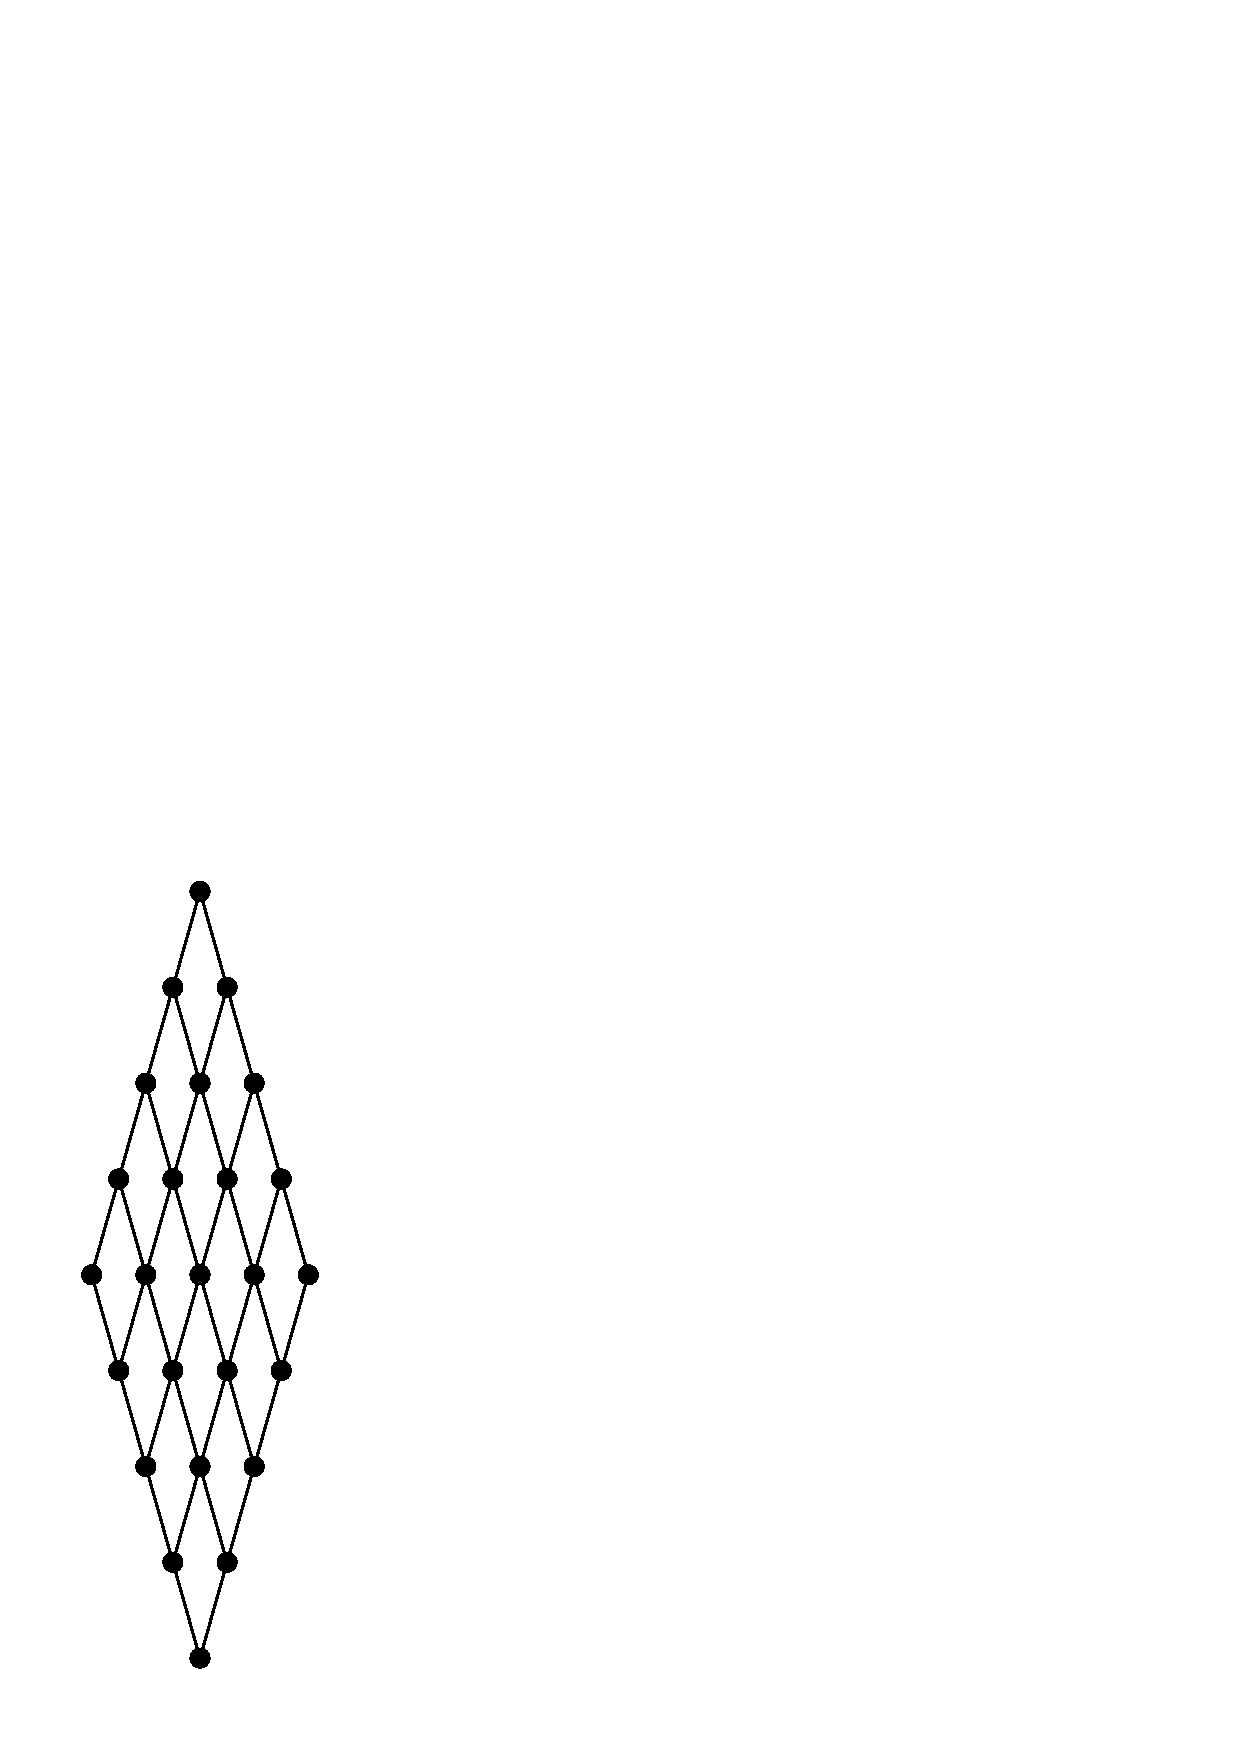
\includegraphics[width=11cm]{resultats/grille55.png}

\subsubsection{5x5 toroidal}

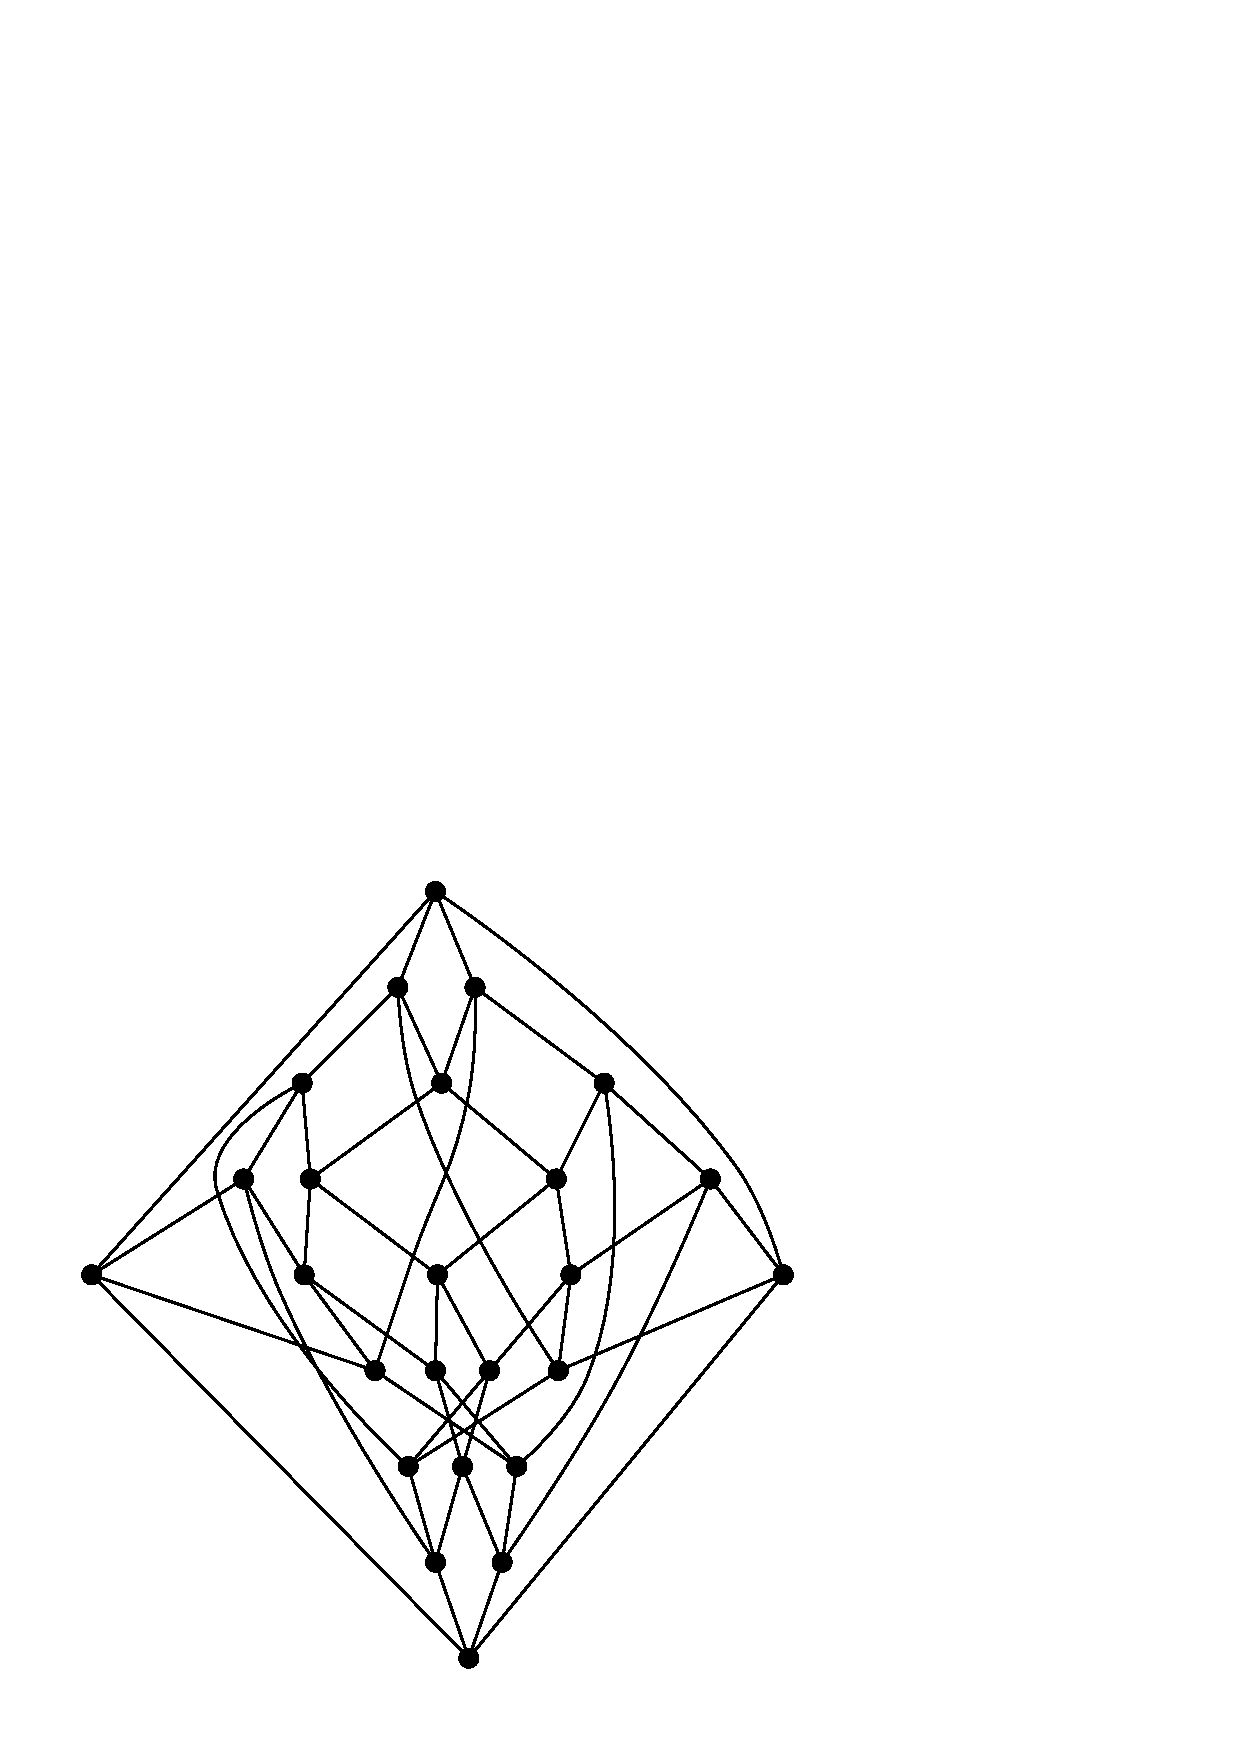
\includegraphics[width=11cm]{resultats/grilletor55.png}

\subsection{Binary Tree}

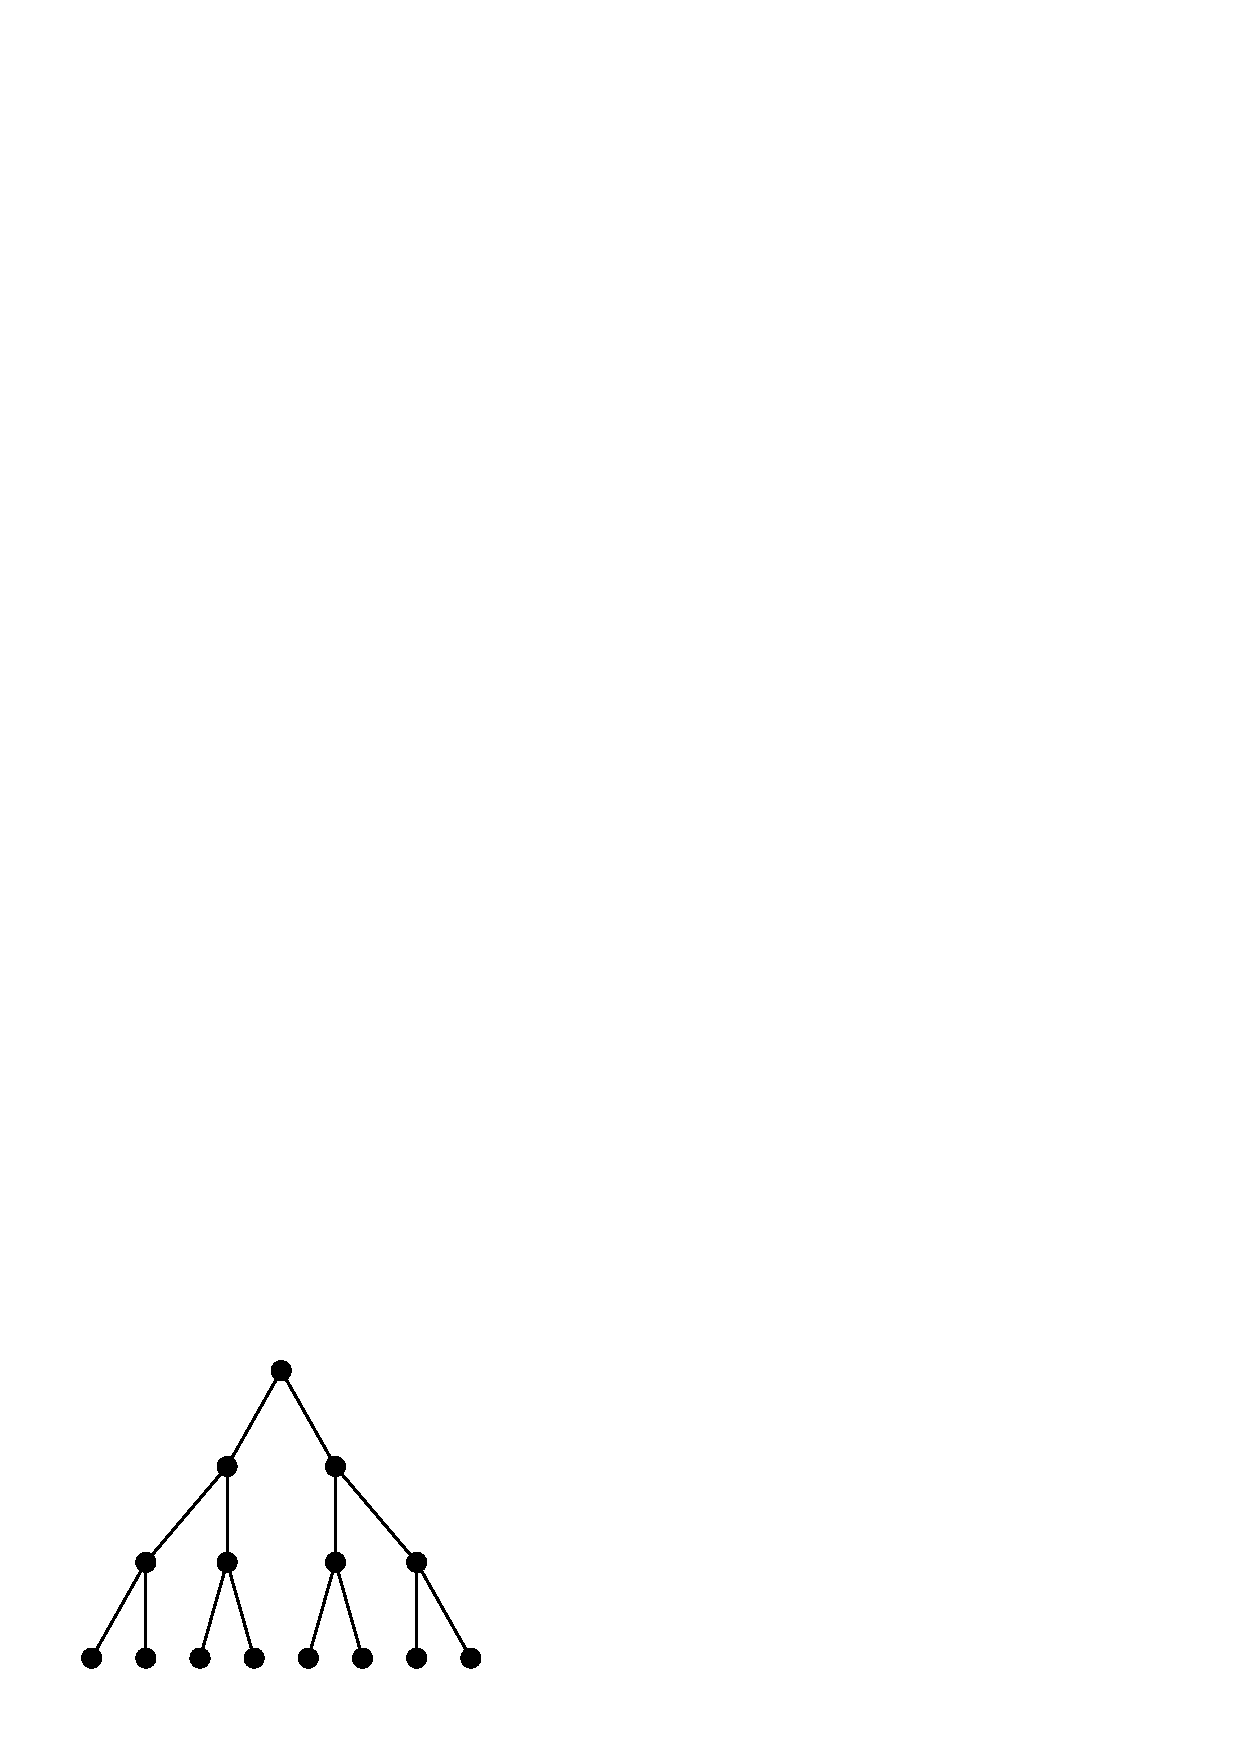
\includegraphics[width=11cm]{resultats/bintree3h.png}

\subsection{Non-Planar Graphs}

\subsubsection{Petersen Graph}


\includegraphics[width=11cm]{resultats/petersen.png}

\subsubsection{Icosaedron Graph}

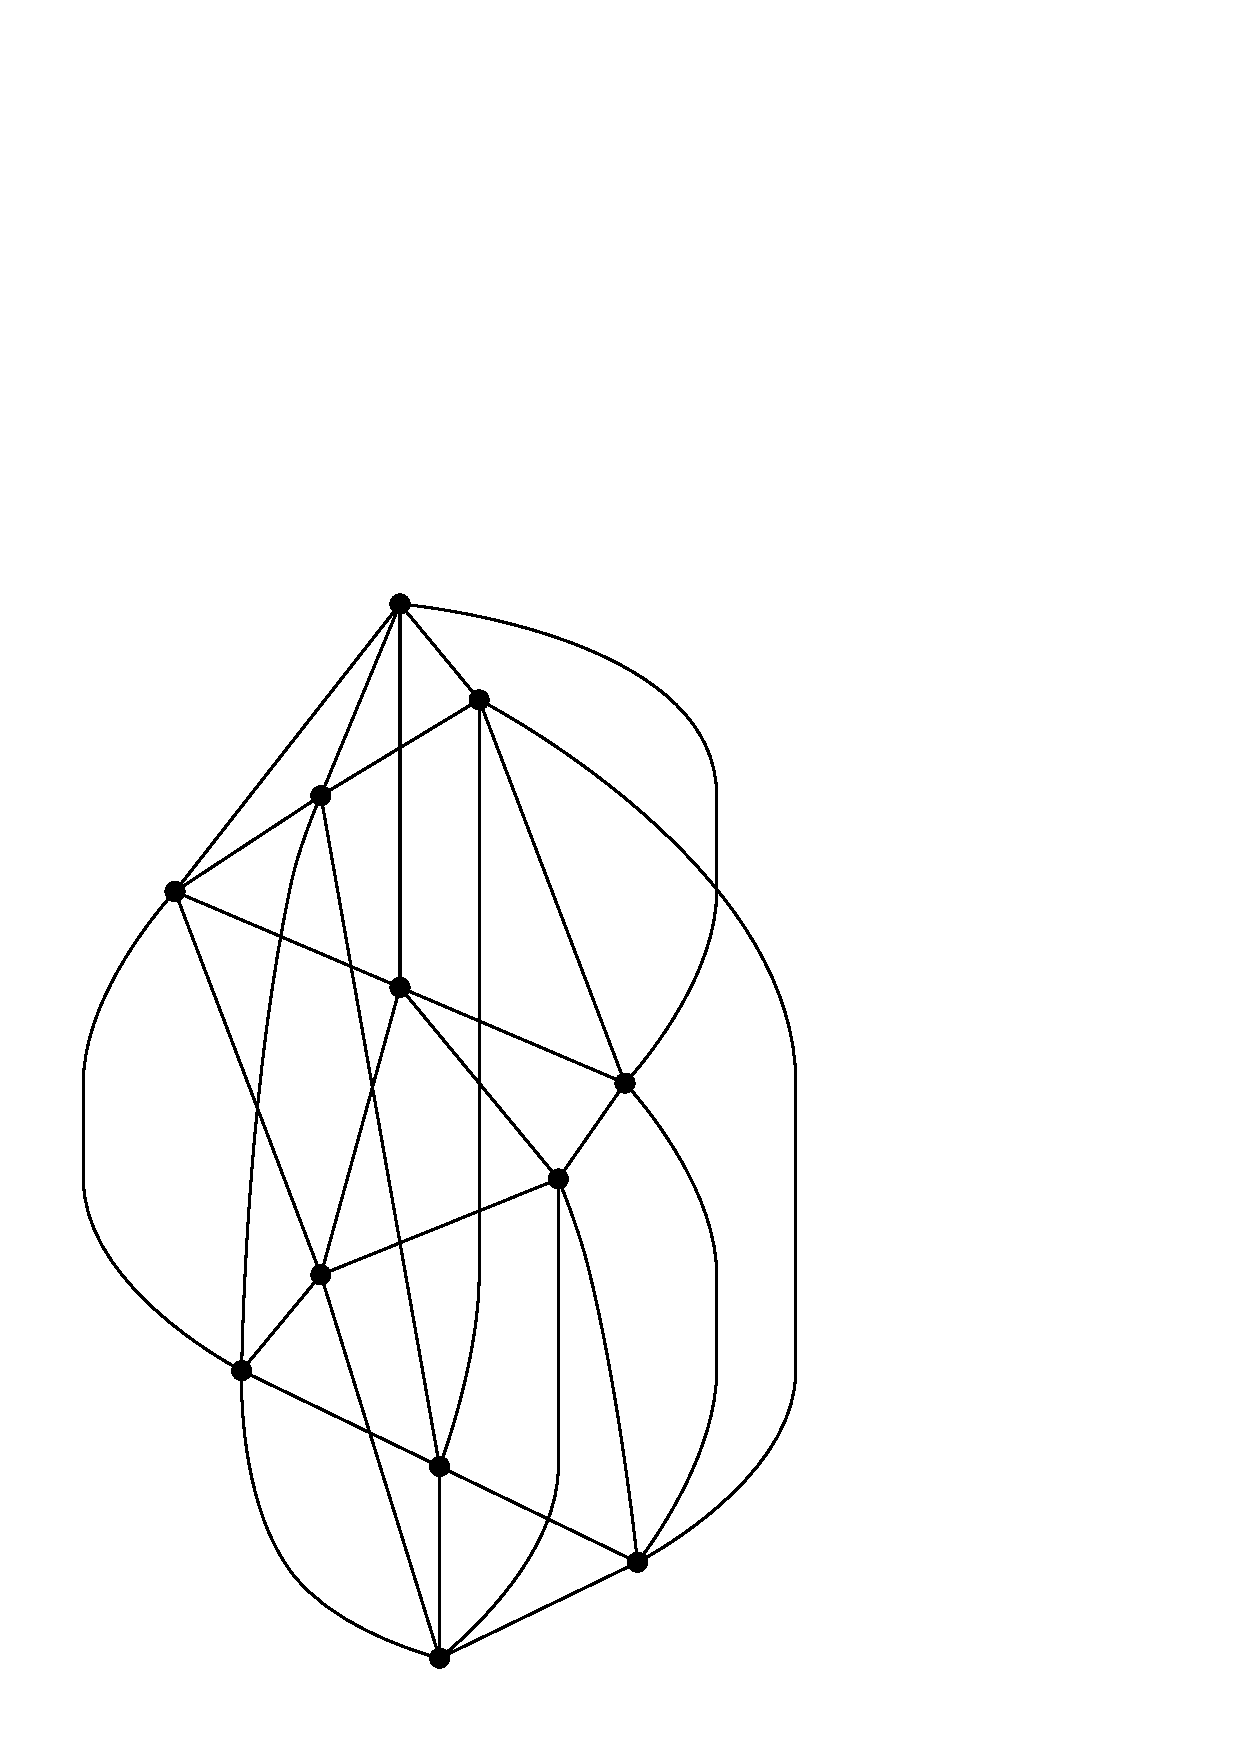
\includegraphics[width=11cm]{resultats/icosaedre.png}

\section{Results summary}

We recall that the game chromatic number of toroidal grids has been proved to be 5 in \cite{Raspaud20091183}. The Grotzsch graph was added later. We were therefore unable to calculate the theoretical values of each strategy in time.\\

\begin{tabular}{|l|c|c|c|c|c|}
\hline 
Graph & Chromatic number & Strategy 1 & Strategy 2 & Strategy 3 & Experimental results \\ 
\hline 
Chain (odd) & 2 & 6 & 6 & 5 & 3 \\ 
\hline 
Chain (even) & 2 & 6 & 6 & 5 & 3 \\ 
\hline 
Cycle (odd) & 3 & 12 & 12 & 8 & 3 \\ 
\hline 
Cycle (even) & 2 & 8 & 12 & 8 & 3 \\ 
\hline 
Grid 2x5 & 2 & 6 & 12 & 5 & 3 \\ 
\hline 
Grid 5x5 & 2 & 10 & 12 & 11 & 5 \\ 
\hline 
Grid 5x5 tor & 3 & 5 & 5 & 5 & 5 \\ 
\hline 
Binary tree & 2 & 6 & 6 & 5 & 4 \\ 
\hline 
Petersen & 3 & 18 & 12 & 14 & 4 \\ 
\hline 
Icosahedron & 4 & 32 & 20 & 20 & 5 \\ 
\hline 
Grotzsch & 4 & ? & ? & ? & 4 \\ 
\hline 
\end{tabular} 
\\
\\
We observe that the experimental values are far below the theoretical values,
especially regarding the Petersen graph and the icosahedron.

 %Expliquer les expériences réalisées, montrer en quoi elles sont pertinentes. Puis montrer quels objectifs ont été atteints. Caractériser le système (sur quoi notre logiciel marche bien, à partir de quand ça se dégrade etc.).
\chapter{Conclusion}
\minitoc

\section{Assessment}

Texte ici.

\subsection{Failures}

Texte ici.



%\section{Si c'était à refaire…}

Si c'était à refaire, nous aborderions le problème différemment...

\section{Prospect}
For a more complete study, it would be interesting to perform simulations on other graphs and to be able to generate the theoretical calculated values on the spot, instead of calculating by hand.


To gain in performances and to accelerate the experiments, we could parallelize the simulations.


It would be interesting to look a little more into Bob's strategies. We considered that Bob and Alice played symmetrically (if a move is bad for Alice, then it is good for Bob), but a bad move for Bob on the short term may be good for him in the end.



\appendix

%\chapter{Diagrammes}

%\section{Architecture}\label{annexe-archi-initiale}


%\chapter{Manuel de maintenance}

%\section{Conventions de codage}\label{annexe-conventions}

\subsection{Langue}

La langue du code doit impérativement être l'Anglais. Les variables, les objets, les classes et les méthodes sont nommés en Anglais.

Les commentaires doivent être écrit de préférence en Anglais. Néanmoins, le Français sera toléré (il vaut mieux écrire quelque chose de compréhensible en Français qu'un truc qui ne veut rien dire en Anglais).

La documentation, elle, est écrite en Français.

\subsection{Forme du code}

\subsubsection{Indentation}

L'indentation doit être effectuée à coup de \textbf{4 espaces}. Ne \textbf{pas} utiliser de tabulation dans le code !

\subsubsection{Opérateurs}

Les opérations utilisant des opérateurs doivent être espacées. De même pour les opérateurs de comparaisons…
Exemple : \verb!toto = tata + titi;! et non pas \verb!toto=tata+titi;! 

\subsubsection{Blocs}

Les blocs se présentent de la forme suivante (exemple avec un if) :
\begin{verbatim}
if (toto == tata) {
    tutu();
}
\end{verbatim}

\textbf{Aucune} autre forme de présentation n'est acceptée ! Pas de crochet ouvrant à la ligne, par exemple.

\begin{note}
  Les blocs if, for… contenant une seule instruction doivent \textbf{quand même} posséder des accolades. Ceci permet d'ajouter plus simplement des instructions si nécessaire, et le code n'en est que plus lisible, on voit bien la hiérarchie des blocs qui se ferment.
\end{note}

\subsubsection{Instructions ternaires}

Les instructions ternaires sont autorisées. En cas d'écriture complexe (plusieurs instructions imbriquées), un commentaire peut-être laissé en fin de ligne. 
Exemple : 
\begin{verbatim}
toto = (tata == 0)?1:10; // Si tata == 0, toto = 1, sinon, toto = 10
                         // mais ce commentaire n'est vraiment pas utile.
\end{verbatim}

\subsection{Contenu du code}

\subsubsection{Classes et Méthodes}

Afin de respecter les principes d'encapsulation, les attributs des classes doivent autant que possible être protected ou private. Pour y accéder, les classes proposent des accesseurs (setter et getter).

\subsubsection{Constructeurs et Destructeurs}

Toute classe doit posséder un destructeur, même s'il est vide.

\subsubsection{Magic Numbers}

Les « magic numbers » sont à éviter. Par exemple : \verb+if (toto == 4) { }+. D'où sort ce `4' ? C'est un « magic number ». Il vaudra donc mieux le remplacer par une constante globale, voire par un \#define, pour savoir à quoi il correspond et pouvoir paramétrer la classe simplement.
Exemple plus lisible :
\begin{verbatim}
#define MAX_THREADS 4
// blabla
if (toto == MAX_THREADS) { } 
\end{verbatim}

\begin{note}
Il peut bien sûr y avoir des exceptions. Les valeurs de 0 et de 1 sont parfaitement tolérées, par exemple.
\end{note}

\subsubsection{Mot clé const}

\begin{itemize}
  \item Si une méthode ne modifie pas l'objet lorsqu'elle est appelée, elle \textbf{doit} être déclarée \verb+const+.
  \item Si un argument d'une méthode n'est pas modifié dans la méthode, il \textbf{doit} être déclaré \verb+const+.
  \item Si un argument d'une méthode est succeptible d'être un gros objet, il devrait généralement être passé par référence constante, et non par copie (exemple : \verb+void setName(string const& name);+).
\end{itemize}

Ces règles permettent d'améliorer significativement la qualité du programme en fournissant des informations importantes au compilateur, mais aussi aux développeurs.

\subsection{Nomage}

Les noms sont tous donnés en anglais, donc la phrase qui suit ne devrait pas être précisée, mais on ne sait jamais… 
\textbf{Jamais}, sous \textbf{aucun} prétexte, d'accent dans le code !

Les variables, objets, classes, fonctions, méthodes… sont nommées de la manière suivante :

\begin{itemize}
  \item \verb+ClassName+
  \item \verb+methodName+
  \item \verb+objectName+ ou \verb+objectname+ (suivant le cas, par exemple, filename est plus joli que fileName).
  \item \verb+CONSTANT_NAME+
  \item \verb+setAttribute+
  \item \verb+getAttribute+
  \item \verb+isAttributed+ (exemple : si l'attribut "enable" est un booléen, \verb+isEnabled()+)
\end{itemize}

\subsubsection{Fichiers}

Les fichiers sont nommés en minuscules, sans espace ni underscore, et se terminent par .h, .cpp.

Par exemple, la classe \verb+ClassName+ sera donc contenue dans les fichiers \verb+classname.h+ et \verb+classname.cpp+. 

\subsection{Commentaires}

Il y a deux types de commentaires.

\subsubsection{Doxygen}

Chaque classe, chaque méthode et chaque slot doivent être documentés à l'aide de Doxygen. 

\subsubsection{Gotcha Keywords}

Le code doit, à chaque fois que c'est nécessaire, contenir des « Gotcha Keywords ». Ces commentaires sont de la forme :
\begin{verbatim}
// :KEYWORD:pseudo:date: commentaire
// Suite du commentaire, si nécessaire
\end{verbatim}

\begin{description}
  \item[KEYWORD] peut être un mot clé dans la liste suivante : DOC, TRICKY, COMMENT, TODO, KLUDGE, WARNING, DEBUG, BUG, DEBUG
  \item[pseudo] est le pseudo de l'utilisateur qui pose le commentaire
  \item[date] \textbf{doit impérativement} être écrite de la forme YYMMDD. Par exemple, pour le 31 février 2012, la date sera 120231
\end{description}

Exemple de gotcha : 
\begin{verbatim}
// :TODO:cbadiola:130115: We must send the report! If we don't, we will get punished!
\end{verbatim}

Un script python\footnote{\url{http://git.meowstars.org/cgit.cgi/gotcha}} permet de sortir la synthèse des GOTCHA de tout un répertoire, très pratique lors de la phase de développement pour avoir une vision globale. N'hésitez donc pas à user et abuser de ce type de commentaires, et choisissant autant que possible le bon mot clé. 


%\chapter{Extraits de code}

%\input{sections/annexe_bidule}


\backmatter

\nocite{*}
\bibliographystyle{alpha}
\bibliography{../refs.bib}

\listoffigures

\listoftables

%\tableofcontents

\newpage
\pagestyle{empty}

Studies and research project report.\\
The map coloring game.\\
Master 2, 2012

\vfill

The sources of this report are freely available on \url{http://github.com/AlexPerrot/map-coloring}.

\bigskip

%Certaines images illustrant ce document sont extraites de nomdusite (\url{http://}). Elles sont disponibles sous licence Creative Commons ou dans le domaine public.

\end{document}
